\documentclass[12pt]{article}

\usepackage{amsmath}
\usepackage{graphicx}
\usepackage{enumerate}
\usepackage{natbib}
\usepackage{url} % not crucial - just used below for the URL 
\usepackage{color}
 \usepackage{multirow}
\newcommand{\todo}[1]{{\color{red}{TO DO: \sc #1}}}

%\pdfminorversion=4
% NOTE: To produce blinded version, replace "0" with "1" below.
\newcommand{\blind}{0}

% DON'T change margins - should be 1 inch all around.
\addtolength{\oddsidemargin}{-.5in}%
\addtolength{\evensidemargin}{-.5in}%
\addtolength{\textwidth}{1in}%
\addtolength{\textheight}{1.3in}%
\addtolength{\topmargin}{-.8in}%

\pdfminorversion=4

\begin{document}

%\bibliographystyle{natbib}

\def\spacingset#1{\renewcommand{\baselinestretch}%
{#1}\small\normalsize} \spacingset{1}


%%%%%%%%%%%%%%%%%%%%%%%%%%%%%%%%%%%%%%%%%%%%%%%%%%%%%%%%%%%%%%%%%%%%%%%%%%%%%%

\if0\blind
{
  \title{\bf A Comparison of Parametric and Permutation Tests for Regression Analysis of Randomized Experiments}
\author{Kellie Ottoboni \\
Department of Statistics; Berkeley Institute for Data Science\\
University of California, Berkeley \\ [.1in]
Fraser Lewis \\
Medical Affairs and Evidence Generation \\
Reckitt Benckiser\\  [.1in]
Luigi Salmaso\\
Department of Management and Engineering \\
University of Padova
}  \maketitle
} \fi

\if1\blind
{
  \bigskip
  \bigskip
  \bigskip
  \begin{center}
    {\LARGE\bf  A Comparison of Parametric and Permutation Tests for Regression Analysis of Randomized Experiments}
\end{center}
  \medskip
} \fi

\bigskip
\begin{abstract}
% 200 words or less
Hypothesis tests based on linear models are widely accepted by organizations that regulate clinical trials.
These tests are derived using strong assumptions about the data-generating process so that the resulting inference can be based on parametric distributions.
Because these methods are well understood and robust, they are sometimes applied to data that depart from assumptions, such as ordinal integer scores.
Permutation tests are a nonparametric alternative that require minimal assumptions which are often guaranteed by the randomization that was conducted.
We compare analysis of covariance (ANCOVA), a special case of linear regression that incorporates stratification, to several permutation tests based on linear models that control for pretreatment covariates.
In simulations using a variety of data-generating processes, some of which violate the parametric assumptions,
the permutation tests maintain power comparable to ANCOVA.
We illustrate the use of these permutation tests alongside ANCOVA with data from a clinical trial comparing the effectiveness of two treatments for gastroesophageal reflux disease.
Given the considerable costs and scientific importance of clinical trials, one may want to include an additional nonparametric method, such as a linear model permutation test, as a robustness check on the statistical inference for the main study endpoints.
\end{abstract}

\noindent%
{\it Keywords:}  Nonparametric methods, linear model, analysis of covariance, analysis of designed experiments
\vfill

\newpage
\spacingset{1.45} % DON'T change the spacing!
\section{Background}
A hypothesis test is a statistical method for determining whether observed data is consistent with a belief about the process that generated the data.
Medical experiments use hypothesis testing to assess the evidence that a treatment affects one or more clinically relevant outcomes.
The simplest version of this experiment involves randomly assigning two treatments to a fixed number of individuals in a group and measuring a single outcome, and has been studied for nearly a century (see \cite{fisher_design_1935} and \cite[1990 translation]{neyman_application_1923} for early references).
One can conduct hypothesis tests and construct confidence intervals for the estimated treatment effect
by exploiting the fact that the difference in average outcomes between the two treatment groups is asymptotically normal with a variance that can be estimated from the data.

Randomized experiments in the real world are rarely this simple:
if individuals are heterogeneous before the study, then their outcomes may differ for reasons besides the treatment;
there may be more than two treatments under study;
patients may not take the treatment they are assigned or may drop out of the study;
and peer effects, the influence of other members of a treatment group, may affect outcomes beyond the treatment itself.
Techniques have been developed to deal with each of these issues, invoking additional assumptions to make valid inference possible.
In this paper, we focus on the issue of heterogeneous pretreatment characteristics and assume that the other issues are not present.

Random assignment of treatment ensures that pretreatment covariates are balanced between treatment groups on average, across all possible randomizations.
However, in any particular randomization, there may be imbalances.
If the imbalanced variables are associated with the outcome, then even when treatment has no effect, there may be differences in outcomes between treatment groups.
Adjusting for such covariates can reduce the variability of treatment effect estimates and yield more powerful hypothesis tests.

Stratification, sometimes called blocking, is one method to control for covariates that are known a priori to be associated with the outcome.
Strata are groups of individuals with similar levels of a covariate.
These groups are defined during the design stage (i.e. before outcome data are collected).
Random assignment of treatments is conducted within each stratum, independently across strata.
This guarantees that the stratification variable is balanced between treatment groups.
A common stratification variable in clinical experiments is location:
individuals often come from many sites because it is difficult to recruit a sufficient number of participants at one doctor's office or hospital,
especially when the object of study is a rare disease or a rare outcome.
Stratification can have the same beneficial effects as controlling for other pretreatment covariates, 
as outcomes may vary across strata due to factors unrelated to individuals' treatment and covariates.

Linear regression is another way to control for imbalanced baseline covariates.
It is done during the data analysis stage.
In its simplest form, linear regression projects the outcomes onto the plane that best summarizes each variable's relationship to the outcome.
The coefficient of any particular covariate answers the question, if we were to hold fixed all other variables and increase this variable by one unit, how much would we expect the outcome to change?
This model posits a linear relationship between covariates, treatment, and outcome; 
if the true relationship is not linear, then linear regression gives the best linear approximation to the conditional expectation of the outcome.
It is standard to use analysis of covariance (ANCOVA) to account for stratification in a linear model.
ANCOVA is a particular case of linear regression that allows the mean outcome to vary from stratum to stratum.
This amounts to fitting a plane to each stratum, with the constraint that they have a common slope.

Hypothesis testing of estimated coefficients requires even stronger assumptions than linearity, namely Gaussian, homoskedastic errors.
When this holds, a regression coefficient scaled by its estimated variance follows Student's $t$ distribution.
Thus, if we believe the linear model is correctly specified, a hypothesis test for a treatment effect amounts to a hypothesis test of the coefficient for treatment in the ANCOVA model, and can be evaluated analytically and efficiently.
However, the modeling assumptions are clearly violated in many cases:
when the data are discrete or ordinal, 
when the treatment has a differential effect across subgroups of individuals and no interaction terms are included, 
and when the variance of outcomes differs across strata.
Furthermore, the hypothesis test implicitly assumes that the data were sampled at random from some underlying population, when in fact,
medical experimenters rarely recruit patients this way (\cite{ludbrook_why_1998}).

Permutation testing is an alternate approach (\cite{fisher_design_1935, pitman_significance_1937,pitman_significance_1938}).
Deliberate randomization induces a distribution for any test statistic under the null hypothesis that treatment has no effect on the outcome:
the randomization scheme provides information about all possible ways that treatment may have been assigned 
and the null hypothesis tells us what each individual's response would be regardless of the assignment (namely, it would be the same).
One determines how ``extreme'' the observed test statistic is relative to this randomization distribution, rather than a parametric reference distribution like Student's $t$ or the standard Gaussian.
Such a test is exact, meaning that it controls the type I error rate at the pre-specified level even in finite samples, whereas parametric hypothesis tests based on asymptotic approximations do not always guarantee good finite sample properties.
Permutation tests condition on the observed sample and do not require any assumptions about the way individuals were sampled from a larger population.
This is useful when the sampling frame is difficult to specify, such as when the study uses a convenience sample.

In the past, statisticians relied on parametric methods because asymptotic approximations were a computationally feasible way to estimate distributions and construct confidence intervals.
Now, computational power is no longer a barrier to finding exact (or exact to pre-specified precision) randomization distributions and confidence intervals.
In most cases, a randomization test is the ``gold standard'':
``[a] corresponding parametric test is valid only to the extent that it results in the same statistical decision [as the randomization test]'' (\cite{bradley_distribution_1968}).
There is no hard and fast rule describing the rate at which parametric tests approach the exact permutation solution, as they are both highly dependent on the particular data observed.
However, if the permutation test agrees with the parametric test, one may have a greater degree of confidence in the estimates and confidence intervals constructed using the parametric method.

We review several hypothesis tests for randomized experiments which adjust for pretreatment covariates to increase power to detect a nonzero treatment effect.  
We focus on ANCOVA and its permutation counterparts, comparing their performance in different scenarios and illustrating their application with a clinical dataset.
Section~\ref{sec:methods} describes the tests and compares their assumptions.
Section~\ref{sec:simulations} presents simulations that suggest that even when assumptions are not satisfied, the parametric and permutation tests have comparable power to detect a treatment effect.
In Section~\ref{sec:results}, we apply each of the tests to data from a clinical trial comparing the performance of two treatments for gastroesophageal reflux disease (GERD).
We conclude in Section~\ref{sec:discussion} with implications of these results for practitioners.

\section{Methods}\label{sec:methods}

\subsection{Notation}
Suppose we have a finite population of $N$ individuals.
Individuals are grouped into strata indexed by $j = 1, \dots, J$, with $n_j$ individuals in stratum $j$ and $\sum_{j=1}^J n_j = N$.
Of the $n_j$ subjects in stratum $j$, $n_{tj}$ are assigned treatment 1, while the remaining $n_j - n_{tj}$ are assigned treatment 0.
Let $Z_{ij}$ indicate the treatment assigned to individual $i$ in stratum $j$.

All individuals have two potential outcomes, $Y_{ij}(1)$ and $Y_{ij}(0)$, representing their responses to treatments $1$ and $0$, respectively.
We can never observe both; random assignment of treatment reveals $Y_{ij} = Z_{ij}Y_{ij}(1) + (1-Z_{ij})Y_{ij}(0)$.
Throughout, we assume that there is no interference between individuals 
(in other words, $Y_{ij}$ is a function of $(Z_{ij}, Y_{ij}(1), Y_{ij}(0))$ and not any other $Z_{i', j'}$ for $(i', j') \neq (i, j)$)
and that there is no censoring or non-compliance
(we actually observe $Y_{ij} = Y_{ij}(Z_{ij})$ for all $(i, j)$).

Furthermore, we observe a covariate $X_{ij}$ that may be associated with the outcome.
For expository clarity, we suppose that $X$ is univariate, but all results are easily extended to the case when $X$ is multivariate.
Suppose further that there is a categorical pretreatment variable with $J$ levels used to stratify individuals. 

We are interested in the effect of treatment, measured as differences in potential outcomes $Y_{ij}(1) - Y_{ij}(0)$.
We may never learn this difference for any particular individual.
However, a tractable problem is to estimate the mean difference in some group, such as the study sample or in a target population.
The chosen method of analysis determines which function of differences is considered.
Various functions of potential outcomes may be of clinical interest; which one prefers depends on the goal of the study.

We study hypothesis testing for whether these differences are nonzero using parametric ANCOVA and its permutation counterparts, assuming this potential outcomes framework throughout.
Other valid methods for comparing two groups include using a two-sample $t$-test to test the difference in two means from normal distributions,
the Wilcoxon rank sum test to test for differences in the medians of two independent groups, 
and the Kolmogorov-Smirnov test and receiver operating characteristic curve analyses to test whether two groups have different distribution functions (\cite{lehmann_nonparametrics_1975,  vexler_statistical_2016}).
We focus on testing using the linear model as this is standard in clinical trials, requires fewer distributional assumptions on the data when using the potential outcomes framework, and incorporates control variables to increase power.


\subsection{Parametric ANCOVA}\label{subsec:ancova}

ANCOVA is based on a linear model with an indicator variable for membership in each stratum.
The model is

\begin{equation}\label{eqn:ancova}
Y_{ij} = \alpha_j + \beta X_{ij} + \gamma Z_{ij} + \varepsilon_{ij}
\end{equation}

\noindent where $\alpha_j$ is a fixed effect for stratum $j$, $\beta$ is the coefficient for the pretreatment covariate,
$\gamma$ is the coefficient for treatment,
and $\varepsilon_{ij}$ is an error term.
The parameter of interest is $\gamma$, and the parametric ANCOVA tests the null hypothesis $H_0: \gamma = 0$ against
the two-sided alternative hypothesis $H_1: \gamma \neq 0$.
If the linear model is the true data-generating process, then $Y_{ij}(1) = Y_{ij}(0) + \gamma$ for all $(i, j)$.
However, we needn't take this perspective for $\gamma$ to be a useful quantity; it represents the average treatment effect, holding the other variables fixed.



To carry out the standard parametric hypothesis test for a linear model, the following assumptions are needed (\cite{freedman_statistical_2005}):
\todo{CHECK}
\begin{enumerate}
\item \textbf{Linearity:} The data $Y$ are related to $X$ and $Z$ linearly.
\item \textbf{Constant slopes:} Stratum membership only affects the intercept $\alpha_j$, not the slopes $\beta$ and $\gamma$.
\item \textbf{IID Errors:} The $\varepsilon_{ij}$ are independent and identically distributed with mean $0$ and common variance $\sigma^2$.
\item \textbf{Independence:} If $X$ is random, $\varepsilon$ is statistically independent of $X$.
\item \textbf{Normality:} The errors are normally distributed.
\end{enumerate}

\todo{are the estimator, standard error, variance clear here?}
The coefficients are estimated using least squares (or equivalently, by maximizing the likelihood).
The estimated coefficient $\hat{\gamma}$ is the estimated average treatment effect. 
(Note, only Assumptions (1) and (2) are needed to guarantee the existence of a solution.
The solution will be unique as long as there is no linear relationship between $X$, $Z$, and stratum membership.)
This procedure also yields an estimate $\hat{\sigma}_{\hat{\gamma}}^2$ of the variance of $\hat{\gamma}$.
Under the null hypothesis, the test statistic 
$$ T = \frac{\hat{\gamma}}{\sqrt{ \hat{\sigma}_{\hat{\gamma}}^2}}$$
follows the Student $t$ distribution with degrees of freedom equal to the number of observations minus the number of parameters estimated (in this case, $N - J - 2$).
The $p$-value for this hypothesis test is the probability, assuming the null hypothesis of zero coefficient is true, that a value drawn from the $t$ distribution is larger in magnitude than $T$.
This test is equivalent to the $F$-test and the likelihood ratio test assuming the Gaussian model,
and \todo{ cite this? is therefore locally most powerful ????}.

However, in the context of a randomized experiment, these assumptions will not be satisfied.
The estimated treatment effect $\hat{\gamma}$ and nominal standard errors $\hat{\sigma}_{\hat{\gamma}}$ can be severely biased (\todo{cite freedman 2008, lin 2013}).
\todo{Lin 2013} shows that running a regression with a full set of treatment and covariate interaction terms cannot hurt asymptotic precision, and using the Huber-White sandwich standard errors can yield asymptotically valid confidence intervals.
In small samples, the bias may still be substantial.
\todo{cite Sekhon post-stratification} show that post-stratification, estimating treatment effects within groups of similar individuals defined after data are collected, can ameliorate this bias.
This is equivalent to estimating a fully saturated linear model with interaction terms for treatment and stratum membership.
The linear ANCOVA model does not account for variation in the treatment effect across strata in this way;
if the difference in potential outcomes is heterogeneous across strata, then the coefficient $\gamma$ may be attenuated towards 0.


\subsection{Stratified permutation test}\label{subsec:strat_perm_test}
In randomization inference, the only random quantities are those involving $Z$, the vector of treatment assignments.
The exact inference is derived from the randomization distribution of statistics involving $Z$.
In particular, the potential outcomes and covariates $(Y_{ij}(1), Y_{ij}(0), X_{ij})$ are fixed in the finite population under study, while the observed response $Y_{ij}$ changes with $Z_{ij}$.
\todo{cite rosenberg 2002}


Suppose we wish to test the null hypothesis that individual by individual, treatment has no effect.
This is referred to as the ``sharp'' null hypothesis:

$$H_0: Y_{ij}(1) = Y_{ij}(0), \forall i = 1, \dots, n_j, j = 1,\dots, J.$$


Under the null hypothesis, which treatment an individual received amounts to an arbitrary label.
Once we observe one response under a particular treatment, we can impute the other potential outcome; namely, it would have been the same.
Thus, the observed $Y_{ij}$ form a sufficient statistic for the data. \todo{cite P\&S}
This null hypothesis is stronger than the null hypothesis for the parametric ANCOVA, which only asserts that differences in potential outcomes are zero \textit{on average}.

In a randomized experiment with complete randomization, any randomization that assigns $n_j$ individuals to treatment 1 in stratum $j$ for each stratum has equal probability.
We can construct the permutation distribution of any statistic under the null hypothesis by imputing the unobserved potential outcomes using the sharp null hypothesis and by re-randomizing treatment assignments using this principle of equal probabilities.
The experimental design specifies the permutation scheme; no additional assumptions are necessary.

The most commonly used statistic is the difference in mean outcomes of subjects who received treatment 1 and the mean outcomes of subjects who received treatment 0.  
This statistic is unbiased over all possible random assignments of treatment which preserve the number of treated individuals,
is interpretable, 
and has convenient theoretical properties owing to it being the difference of two means.
However, the difference in means may not be optimal if we want to detect heterogeneous effects.  
For an extreme example, imagine that the sample contains an equal number of males and females, and each treatment is assigned to half of males and half of females.  
Everybody who receives treatment 0 has an outcome of 0, but males who receive treatment 1 have an outcome of $1$ and females who receive treatment 1 have an outcome of $-1$.  
Then the difference in means between the treatment groups is $0$, even though the treatment had nonzero effects on both males and females.  
This differential effect gets averaged out.

To avoid this, one may want to account for the stratification. 
One way to construct a stratified test is to use the same stratified permutation scheme but a different statistic which combines the stratum-specific statistics into a single value, for instance taking the sum of their absolute values.
Taking the absolute value before summing ensures that effects with different signs do not cancel each other out.
Another way to construct a test is to use the nonparametric combination (NPC) framework proposed by \citet{pesarin_permutation_2010}.
In this framework, the ``global'' null hypothesis of no effect whatsoever is decomposed into the intersection of ``partial'' null hypotheses of no treatment effect within each stratum.
For NPC, one first conducts each partial test separately, then combines their $p$-values in a way that preserves dependencies.
This method is equivalent to combining stratum statistics directly when data are from a randomized experiment, because treatment is independent across strata.


\subsection{Permutation tests with the linear model}\label{subsec:lm_perm_tests}
The tests in Section~\ref{subsec:strat_perm_test} only use information on the treatment and the outcome.
However, experimenters record additional covariates that may be predictive of the outcome.
A test that incorporates these covariates may reduce the variance of the statistic and have more power.
The permutation tests in this section use the linear model in Equation~\ref{eqn:ancova}, but make different assumptions about the data.
In a randomized experiment, the treatment assignment is independent of covariates, errors, and potential outcomes,
making several variables exchangeable.
We show two permutation tests developed in this framework.

The first linear model permutation test is a variation on the stratified permutation test described in Section~\ref{subsec:strat_perm_test}.
The only difference is the test statistic:
this test uses the $t$ statistic for the regression coefficient of $Z$ in the linear model in Equation~\ref{eqn:ancova}.
Rather than using the $t$ distribution to calculate the significance of the observed $t$ statistic, we construct the permutation distribution of the $t$ statistic.
Again, the experimental design specifies the randomization distribution and no additional assumptions are needed:
$Z$ is independent of $(Y(1), Y(0), X)$ conditional on strata.

\citet{freedman_nonstochastic_1983} propose an alternative test based on the residuals of the linear regression.
They take an alternative view of the problem:
instead of assuming the data are generated according to the linear model Equation~\ref{eqn:ancova}, they \textit{define} the errors $\varepsilon_{ij}$ to be the difference between the observed outcome $Y_{ij}$ and the data's linear projection onto the plane $\alpha_j + \beta X_{ij}+ \gamma Z_{ij}$.
The $\varepsilon$ are fixed approximation errors in this framework, not independent and identically distributed random errors.

If the null hypothesis is true, then $\gamma = 0$ and $\varepsilon_{ij} = Y_{ij} - \alpha_{ij} - \beta X_{ij}$ for all $i = 1, \dots, n_j, j = 1, \dots, J$.
Therefore, we may estimate the errors by $\hat{\varepsilon} =Y - \hat{Y}$, where $\hat{Y}$ is the vector of fitted values from the regression of $Y$ on $X$ but not $Z$.
The $\hat{\varepsilon}$ approximate the true errors $\varepsilon$ from the true data-generating process, assuming that the null hypothesis is true.
Furthermore, under the null hypothesis, the $\varepsilon$ are independent of $Z$ within strata. 
Thus, we can carry out an approximate permutation test by permuting the estimated $\hat{\varepsilon}$ within strata, independently across strata.

The test has two important assumptions:
the relationship between $Y$ and $X$ is linear and errors are IID within strata.
Together, these conditions ensure that $\varepsilon$ are exchangeable against $X$ within strata.
In practice, we must estimate $\alpha$; using $\hat{\alpha}$ to estimate $\hat{Y}$ yields an approximate permutation test.
The $\hat{\varepsilon}$ may not even be approximately exchangeable within strata if the regression does not describe the relation between $Y$ and $X$ well.
For this reason, \cite{freedman_nonstochastic_1983} advise against using the method if there are large outlier values in the covariate $X$ or when $X$ and $Z$ are highly colinear.
Randomization does not guarantee this additional exchangeability assumption, so it should be checked.
One way, suggested by \cite{freedman_nonstochastic_1983}, is to visually inspect a scatterplot of the residuals against $X$.
One may also run a hypothesis test for association, such as a stratified permutation test using the correlation as a statistic.
\todo{Do this test in the empirical section}


To summarize the steps for constructing a permutation distribution:

\begin{enumerate}
\item Regress $Y$ on $X$ and stratum indicators, \textit{but not $Z$} to obtain $\hat{Y}$. Estimate the errors by $\hat{\varepsilon} = Y - \hat{Y}$.
\item Permute the $\hat{\varepsilon}$ within strata to obtain permuted errors $\hat{\varepsilon}^\pi$.
\item Construct permuted responses $Y^\pi = \hat{Y}+ \hat{\varepsilon}^\pi$.
\item Regress $Y^\pi$ on $X$, $Z$, and stratum indicators. The test statistic is the $t$ statistic for the coefficient of $Z$.
\end{enumerate}


Others have developed variants on these approximate regression-based permutation tests. 
There is some disagreement on what constitutes an appropriate permutation scheme.
\cite{manly_randomization_2006} proposed randomizing the outcomes $Y$, treating them as though they were randomly assigned to pairs $(X, Z)$ under the null hypothesis.
Permuting data this way corresponds to the null hypothesis that all coefficients are 0 in the linear model, which may not reflect the true relationship between variables.
\cite{kennedy_randomization_1995} proposed a permutation method similar in spirit to \cite{freedman_nonstochastic_1983}, but which differs procedurally.
Both methods attempt to measure the correlation between treatment and unexplained variation in outcomes, but
instead of regressing pseudo-outcomes $Y^\pi$ on covariates to obtain a permutation distribution, \cite{kennedy_randomization_1995} recommends using the $t$ statistic from regressing $Z$ on the permuted residuals $\hat{\varepsilon}^\pi$. 

Several authors have compared these tests theoretically and empirically (\cite{anderson_empirical_1999, anderson_permutation_2001, kennedy_randomization_1996}).
They find that the Freedman-Lane test of residuals is asymptotically equivalent to the ``oracle'' exact hypothesis test which we could conduct if we knew which permutations of $Y$ given $X$ were equiprobable under the null hypothesis (\cite{anderson_permutation_2001}).
This agrees with empirical results, which show that the Freedman-Lane test performs better than other linear model permutation tests in simulations, though its advantage is small (\cite{anderson_empirical_1999}). 
Therefore, throughout the rest of the paper we focus on the two linear regression permutation tests we described in detail: linear regression with permuted treatment assignments and the Freedman-Lane method of permuting residuals.


\section{Simulations}\label{sec:simulations}

We simulated data from a randomized experiment using several different data-generating processes.
We applied the tests to the data and compared their empirical power over repeated random treatment assignments and random errors.
We compared the following five tests:
the $t$ test from the parametric ANCOVA,
a stratified permutation test using the difference in mean outcomes
 (called ``stratified permutation'' in what follows),
a stratified permutation test using the mean change scores, defined as the difference between the baseline measure and the outcome (called ``differenced permutation'' in what follows),
a stratified permutation test based on the $t$ statistic from the linear regression of outcome on control variables (called ``LM permutation'' in what follows),
and the Freedman-Lane permutation test.
The simulations are included in three supplementary files.

\subsection{Continuous outcomes}

In the first set of simulations, we generated continuous potential outcomes.
We used two scenarios.
In the first, the treatment effect was constant across strata.
We drew a latent random variate $v_{ij}$ from the uniform distribution on $[-4, 4]$.
In the second scenario, the treatment effect varied across strata, and we drew the latent random variable according to
\begin{displaymath}
   v_{ij} \sim \left\{
     \begin{array}{lr}
       \text{Unif}[-4, -1] & : j=1\\
       \text{Unif}[-1, 1] & : j=2\\
       \text{Unif}[1, 4] & : j=3\\
     \end{array}
   \right.
\end{displaymath} 

We generated independent and identically distributed errors $\varepsilon_{ij}$ and $\delta_{ij}$ and varied the error distribution. 
The errors were either standard normal (to mimic the usual ANCOVA assumptions),
$t$ distributed with two degrees of freedom,
standard lognormal,
or exponentially distributed, with scale parameter $1$ and shifted to have mean zero.
The observed $(v_{ij}, \varepsilon_{ij}, \delta_{ij})$ were independent across $i$ and $j$.

The baseline value for individual $i,j$ was 
$$ X_{ij} = \frac{\gamma e^{v_{ij}} + e^{v_{ij}/2}}{2} + \varepsilon_{ij}$$.

Then we generated potential outcomes as

$$Y_{ij}(Z_{ij}) = \frac{(2Z_{ij} - 1)\gamma e^{v_{ij}} + e^{v_{ij}/2}}{2} + \delta_{ij}.$$

The treatment effect for individual $(i, j)$ is $\gamma e^{v_{ij}}$ and we would like to estimate the average treatment effect in the sample.

Assume that there are $n_j=16$ individuals per stratum and treatment assignment is balanced, i.e. 8 people receive each treatment at each stratum.
After sampling $(v_{ij}, \varepsilon_{ij}, \delta_{ij})$, we regenerate $Z$ and the potential outcomes $Y(Z)$ 10,000 times.
We repeat this procedure for each distribution of latent variables $v$ and of the errors $\varepsilon$ and $\delta$.

\todo{insert figures and table}


\todo{what's the correlation between $X$ and $Y$?}
\subsection{Discrete outcomes}

\subsection{Imbalanced treatment groups}
%Outcomes were generated according to the linear equation 
%\begin{equation}\label{eqn:dgp}
%Y_{ij1} =\alpha_j + \beta_0Y_{ij0} + \gamma_j Z_{ij} + \varepsilon_{ij}
%\end{equation}
%
%\noindent for individuals $i = 1, \dots, n_j$, $j = 1, 2, 3$.
%$\alpha_j$ is the mean effect of being in stratum $j$, 
%$\beta_0$ is the coefficient for the baseline measurement $Y_{ij0}$, 
%$Z_{ij}$ is the treatment level, 
%$\gamma_j$ is the effect of treatment in stratum $j$, 
%and $\varepsilon_{ij}$ is an error term.
%We used three strata with $\alpha_1 = 1, \alpha_2 = 1.5,$ and $\alpha_3 = 2$.
%
%We used two designs:
%\begin{itemize}
%\item Constant additive treatment effect: $\gamma_1 = \gamma_2 = \gamma_3 = \gamma$. This is the implicit assumption when using a linear model.
%\item Treatment effect in a single stratum: $\gamma_1 = \gamma > 0$, $\gamma_2 = \gamma_3 = 0$. This is a constant, additive treatment effect in stratum 1, but no treatment effect in strata 2 and 3. This is a simplistic example of a heterogeneous treatment effect. The standard ANCOVA model does not account for this scenario.
%\end{itemize}
%
%\noindent We drew the baseline measurements once, treating them as fixed, and conditioned on observing $\{ Y_{ij0} : {i = 1,\dots,n_j, j = 1,\dots, 3}\}$.
%We randomly assigned treatment to half of the individuals within each stratum, generated random errors, and constructed new outcomes $Y_{ij1}$ using Equation~\ref{eqn:dgp}.
%We conducted all five tests on this new data, obtaining a two-sided $p$-value for each.
%We repeated these steps using the same $\{ Y_{ij0} \}$ 1000 times.
%
%In our first set of simulations, we assumed that the baseline measurements $Y_{ij0}$ were standard normally distributed and the pairs $(Y_{ij0}, \varepsilon_{ij})$ were independent across $i$ and $j$.
%We let $\beta_0 = 1$ and the treatment effect be $\gamma = 1$.
%We used a balanced design with $n_j = 16$ individuals per stratum and balanced treatment assignment, i.e. 8 subjects received each treatment within each stratum.
%There were four total simulation designs:
%for each of the two possible treatment effects, we used two distributions for $\varepsilon$.
%In the first case, we used $\varepsilon \sim N(0, 1)$ to match the parametric assumption of normal errors.
%In the second case, $\varepsilon$ were drawn from a $t$ distribution with 2 degrees of freedom so the errors were heavy-tailed.
%
%Figure~\ref{fig:normal_sim_power} shows the estimated power curves in these four designs.
%The best case was when the errors were Gaussian and the treatment effect was constant across strata, while the worst case was when the errors are heavy-tailed and the treatment effect only appeared in one stratum.
%Intuitively, it makes sense that power decreased relative to the Gaussian, constant treatment effect case, as each violated assumption further obscured the treatment effect.
%A consistent pattern appeared in each design: the stratified permutation test had the lowest power, while the other four tests tended to have similar power.
%
%Table~\ref{tab:normal_power} displays the size of the test and the power at level $0.05$.
%The three tests based on linear models had slightly higher than nominal level, though the margin was within two standard errors of $0.05$.
%(The number of tests rejected under the null in 1000 trials has a binomial distribution.
%If the true level is $0.05$, then the standard error is $\sqrt{0.05 \times 0.95/1000}$.)
%These numbers show that actually, for $\alpha=0.05$, the stratified permutation test did not lose a large amount of power when the effect was isolated in a single stratum.
%In this case, the stratified permutation test may have slightly higher power than ANCOVA at the small significance levels typically used in practice.
%\begin{figure}[h]
%\centering
%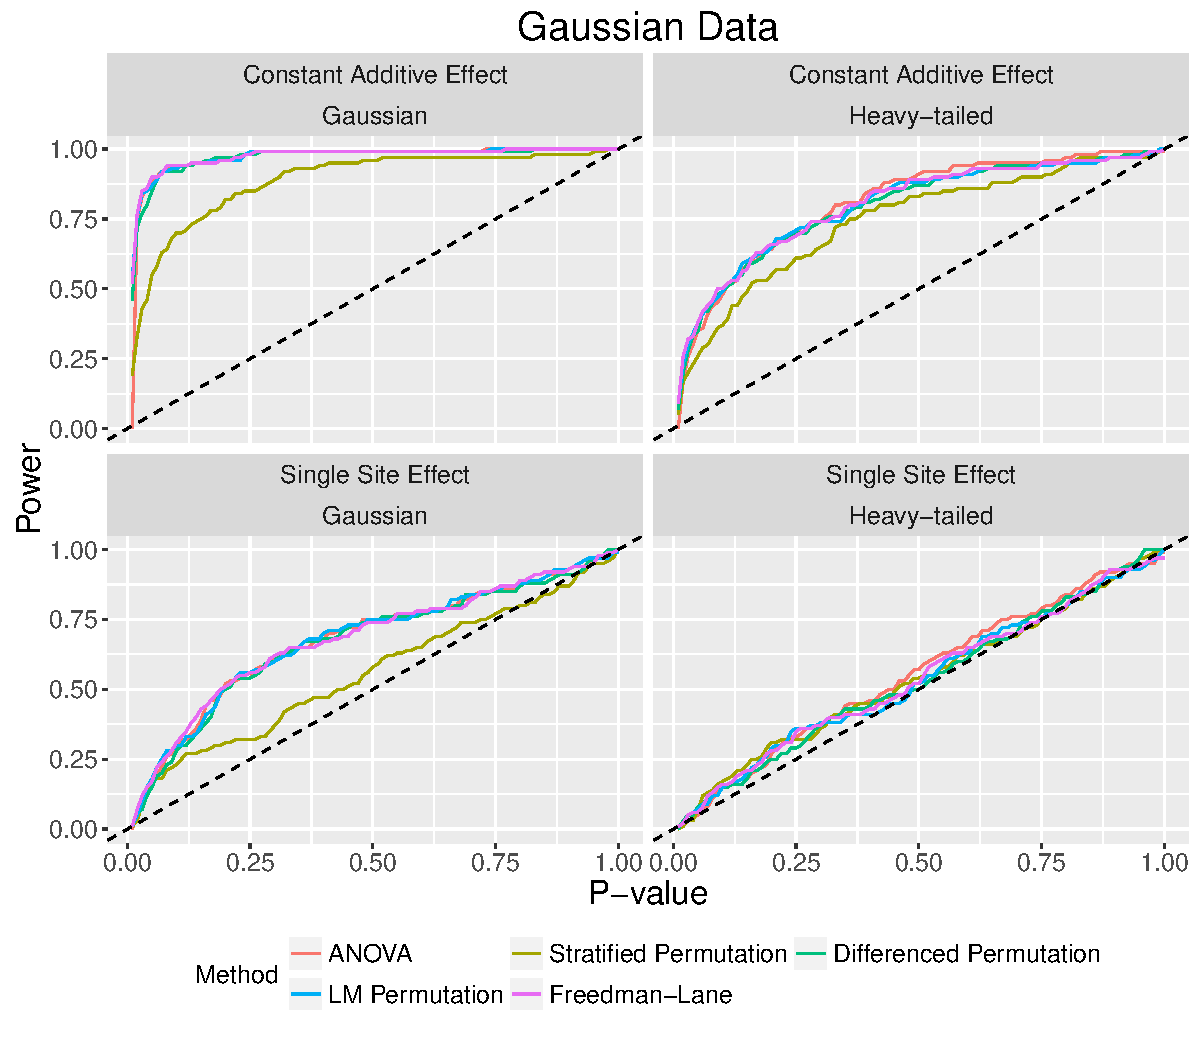
\includegraphics[width = \textwidth]{fig/normal_simulation_power.pdf}
%\caption{Empirical power curves for the Gaussian simulated data}
%\label{fig:normal_sim_power}
%\end{figure}
%%\begin{center}
%%\begin{table}[ht]
\centering
\begin{tabular}{p{1.15in}|p{0.7in}|p{0.6in}p{0.8in}p{0.8in}p{0.8in}p{0.75in}}
  \hline
Treatment & Errors & ANOVA & Stratified Permutation & Differenced Permutation & LM Permutation & Freedman-Lane \\ 
  \hline
Constant Additive Effect & Gaussian & 0.89 & 0.55 & 0.86 & 0.89 & 0.89 \\ 
  Single Stratum Effect & Gaussian & 0.16 & 0.09 & 0.16 & 0.16 & 0.17 \\ 
  Constant Additive Effect & Heavy-tailed & 0.35 & 0.24 & 0.38 & 0.40 & 0.39 \\ 
  Single Stratum Effect & Heavy-tailed & 0.07 & 0.08 & 0.08 & 0.08 & 0.08 \\ 
   \hline
\end{tabular}
\caption{Empirical power at level $0.05$ for Gaussian simulated data} 
\label{tab:normal_power}
\end{table}

%%\end{center}
%
%
%
%\begin{table}[]
%\centering
%\begin{tabular}{ll|ccccc}
%\multicolumn{2}{c|}{Design}                                                                  & \multicolumn{5}{c}{$p$-value}                                                                                                                                                                                                                                                                                                                                           \\ \hline
%Errors                        & \begin{tabular}[c]{@{}l@{}}Treatment \\ Effect\end{tabular} & \multicolumn{1}{l}{ANCOVA} & \multicolumn{1}{l}{\begin{tabular}[c]{@{}l@{}}Stratified\\ Permutation\end{tabular}} & \multicolumn{1}{l}{\begin{tabular}[c]{@{}l@{}}Differenced\\ Permutation\end{tabular}} & \multicolumn{1}{l}{\begin{tabular}[c]{@{}l@{}}LM\\ Permutation\end{tabular}} & \multicolumn{1}{l}{\begin{tabular}[c]{@{}l@{}}Freedman-\\ Lane\end{tabular}} \\ \hline
%\multirow{3}{*}{Gaussian}     & None                                                        & 0.058                      & 0.042                                                                                & 0.038                                                                                 & 0.062                                                                        & 0.057                                                                        \\
%                              & Constant                                                    & 0.886                      & 0.545                                                                                 & 0.858                                                                                 & 0.891                                                                        & 0.892                                                                        \\
%                              & Single stratum                                              & 0.159                      & 0.089                                                                                & 0.160                                                                                 & 0.162                                                                        & 0.170                                                                        \\ \hline
%\multirow{3}{*}{Heavy-tailed} & None                                                        & 0.032                      & 0.040                                                                                & 0.045                                                                                 & 0.042                                                                        & 0.040                                                                        \\
%                              & Constant                                                    & 0.355                      & 0.240                                                                                & 0.378                                                                                 & 0.400                                                                        & 0.393                                                                        \\
%                              & Single stratum                                              & 0.066                      & 0.080                                                                                & 0.082                                                                                 & 0.076                                                                        & 0.080                                                                        \\ \hline
%\end{tabular}
%\caption{Empirical power at level $0.05$ for Gaussian simulated data with balanced treatment groups.}
%\label{tab:normal_power}
%\end{table}
%
%Our second set of simulations used the same design as the previous ones, but modified the sizes of the treatment groups.
%Within each stratum, 4 individuals received one treatment and 12 received the other.
%This mimics some real-world experiments, where the more expensive treatment is administered less frequently than the placebo or standard of care.
%It is well-known that both parametric and nonparametric tests have higher than nominal level when there is heterogeneous variance, and this effect is exacerbated when group sizes are unequal (\cite{glass_consequences_1972}, \cite{zimmerman_two_2006}).
%Here, the data had equal variances so we would expect power, not the test level, to be an issue.
%(See the supplementary Gaussian simulations for simulations using data with heterogeneous variances.)
%Table~\ref{tab:imbalanced_power} displays the value of these power curves and the size of the test at level $0.05$.
%In this case, the permutation tests (except for the simple stratified permutation) had slightly higher power than ANCOVA, but the difference was not substantial.
%
%%\begin{center}
%%\begin{table}[ht]
\centering
\begin{tabular}{|p{0.7in}|p{0.6in}p{0.8in}p{0.8in}p{0.8in}p{0.8in}p{0.75in}}
  \hline
Treatment & Errors & ANCOVA & Stratified Permutation & Differenced Permutation & LM Permutation & Freedman-Lane \\ 
  \hline
No Effect & Gaussian & 0.046 & 0.031 & 0.028 & 0.042 & 0.045 \\ 
  Constant Additive Effect & Gaussian & 0.840 & 0.490 & 0.810 & 0.870 & 0.860 \\ 
  Single Stratum Effect & Gaussian & 0.120 & 0.050 & 0.090 & 0.100 & 0.120 \\ 
   \hline
No Effect & Heavy-tailed & 0.034 & 0.054 & 0.055 & 0.047 & 0.042 \\ 
  Constant Additive Effect & Heavy-tailed & 0.230 & 0.200 & 0.270 & 0.260 & 0.270 \\ 
  Single Stratum Effect & Heavy-tailed & 0.070 & 0.080 & 0.090 & 0.090 & 0.080 \\ 
   \hline
\end{tabular}
\caption{Empirical power at level $0.05$ for Gaussian simulated data with imbalanced treatment groups} 
\label{tab:imbalanced_power}
\end{table}

%%\end{center}
%
%
%\begin{table}[ht]
%\centering
%\begin{tabular}{ll|ccccc}
%\multicolumn{2}{c|}{Design}                                                                 & \multicolumn{5}{c}{$p$-value}                                                                                                                                                                                                                                                                                                                                           \\ \hline
%Errors                        & \begin{tabular}[c]{@{}l@{}}Treatment \\ Effect\end{tabular} & \multicolumn{1}{l}{ANCOVA} & \multicolumn{1}{l}{\begin{tabular}[c]{@{}l@{}}Stratified\\ Permutation\end{tabular}} & \multicolumn{1}{l}{\begin{tabular}[c]{@{}l@{}}Differenced\\ Permutation\end{tabular}} & \multicolumn{1}{l}{\begin{tabular}[c]{@{}l@{}}LM\\ Permutation\end{tabular}} & \multicolumn{1}{l}{\begin{tabular}[c]{@{}l@{}}Freedman-\\ Lane\end{tabular}} \\ \hline
%\multirow{3}{*}{Gaussian}     & None                                                        & 0.046                      & 0.031                                                                                & 0.028                                                                                 & 0.042                                                                        & 0.045                                                                        \\
%                              & Constant                                                    & 0.840                      & 0.490                                                                                & 0.810                                                                                 & 0.870                                                                        & 0.860                                                                        \\
%                              & Single stratum                                              & 0.120                      & 0.050                                                                                & 0.090                                                                                 & 0.100                                                                        & 0.120                                                                        \\ \hline
%\multirow{3}{*}{Heavy-tailed} & None                                                        & 0.034                      & 0.054                                                                                & 0.055                                                                                 & 0.047                                                                        & 0.042                                                                        \\
%                              & Constant                                                    & 0.230                      & 0.200                                                                                & 0.270                                                                                 & 0.260                                                                        & 0.270                                                                        \\
%                              & Single stratum                                              & 0.070                      & 0.080                                                                                & 0.090                                                                                 & 0.090                                                                        & 0.080                                                                        \\ \hline
%\end{tabular}
%\caption{Empirical power at level $0.05$ for Gaussian simulated data with imbalanced treatment groups.} 
%\label{tab:imbalanced_power}
%\end{table}
%
%In our third set of simulations, we made the baseline measurements $Y_{ij0}$ discrete and skewed.
%This type of data may occur in surveys where individuals are asked to rate their symptom severity on a discrete ordinal scale.
%We generated the baseline measures using independent draws from a Poisson distribution with mean 4 and censored values at 10.
%We conditioned on these observed baseline measures after generating them once.
%Then, for each of 1000 trials, we randomly assigned treatment to half of the individuals in each stratum and generated errors taking on values $0.5$ and $-0.5$ with equal probability.
%We constructed $Y_{ij1}$ using Equation~\ref{eqn:dgp} with a treatment effect of $\gamma = 0.5$.
%To ensure that both baseline and outcome were integer scores, we let the $Y_{ij1}$ be unobservable and defined the observed outcome as
%
%\begin{displaymath}
%   \tilde{Y}_{ij1} = \left\{
%     \begin{array}{ll}
%       1 & \text{if } {Y}_{ij1} < 1\\
%       10 & \text{if } {Y}_{ij1} > 10 \\
%       \lfloor {Y}_{ij1} \rfloor & \text{otherwise}
%     \end{array}
%   \right.
%\end{displaymath}
%
%
%The observed outcomes $\tilde{Y}_{ij1}$, the baseline measures $Y_{ij0}$, and the errors were discrete, violating normality assumptions.
%
%We examined the effect of stratum size in this set of simulations.
%For each of the two treatment effect designs, we considered both equal and unequal stratum sizes.
%The simulations with equal stratum sizes were generated as before, where each stratum contained $n_j = 16$ individuals.
%The simulations with unequal stratum sizes were set up so the smallest stratum had only $n_1=8$ individuals, the next had $n_2= 16$, and the largest had $n_3=24$.
%The design with a nonzero treatment effect in a single stratum and unequal stratum sizes was particularly unfavorable:
%the nonzero effect only occurred in the smallest stratum.
%
%Figure~\ref{fig:skewed_sim_power} shows the estimated power curves in these four designs.
%When the treatment effect was constant, sample sizes within each stratum didn't matter; 
%the two power curve plots in the first row of Figure~\ref{fig:skewed_sim_power} look the same up to chance variation.
%When the treatment effect only occurred in one stratum, there was a substantial loss in power.
%It was nearly impossible to detect a difference in treatments when the affected stratum was too small.
%In practice, one does not usually know a priori which individuals will be affected by treatment (otherwise, those not affected would be excluded from the study altogether).
%This result suggests that when stratifying, one must be cautious not to stratify too finely, as it is impossible to measure an effect with an insufficient sample size.
%
%All of the tests appeared to be conservative and to have lower than nominal level.
%As in the first set of simulations, the stratified permutation test using the raw outcomes had the lowest power of the five tests.
%The stratified permutation test using the change scores also had lower power than the three linear model tests.
%Presumably, this was because the differences $\tilde{Y}_{ij1} - Y_{ij0}$ were discrete and limited to a small number of values, so the test statistic could not vary greatly across permutations.
%Table~\ref{tab:skewed_power} confirms this: power for the three linear model methods was high when the treatment was constant across strata, and power for all of the methods suffered when the effect was isolated in a single stratum.
%
%
%\begin{figure}
%\centering
%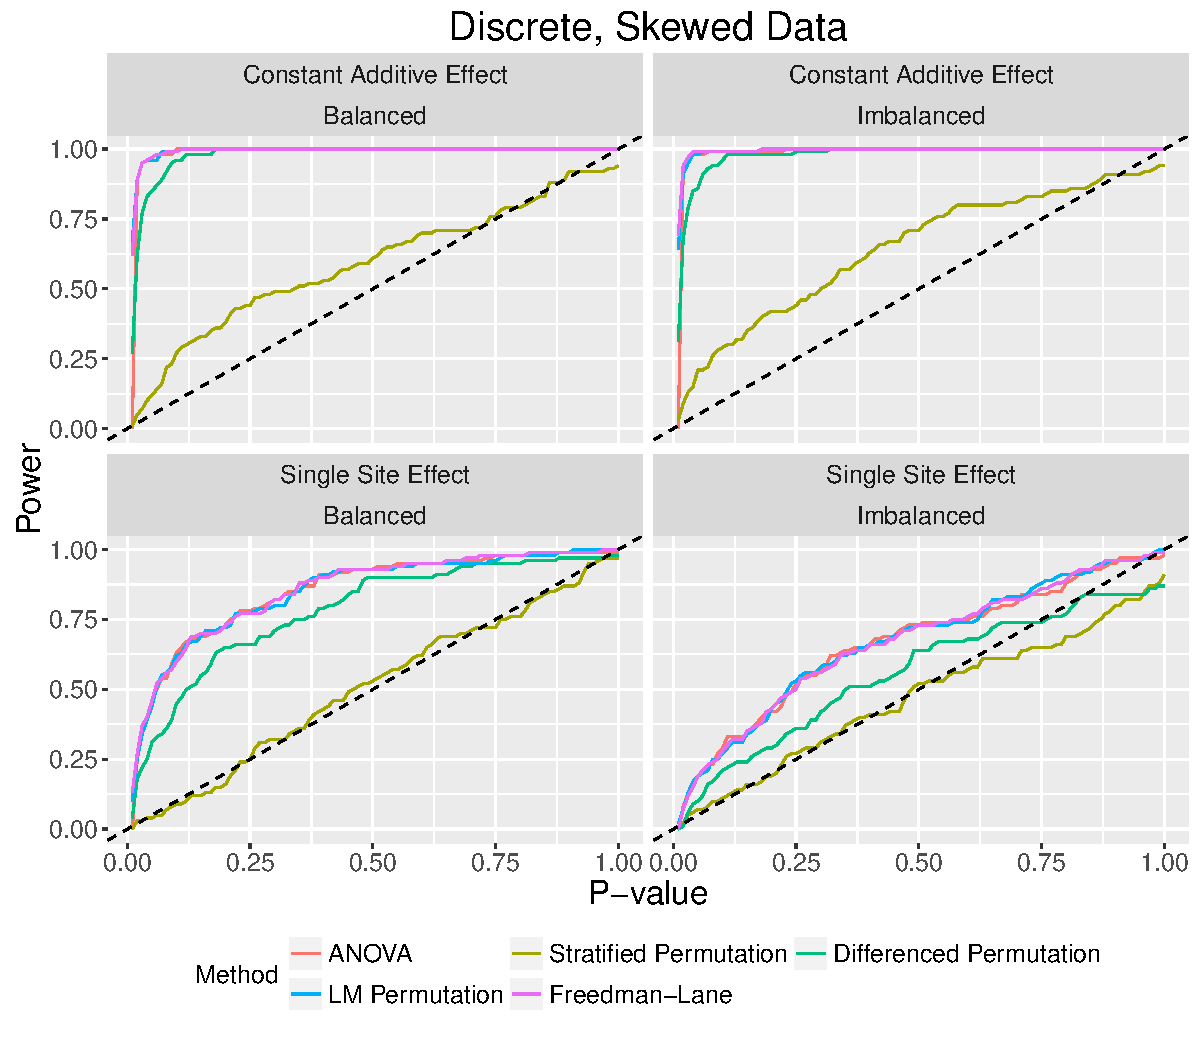
\includegraphics[width = \textwidth]{fig/skewed_simulation_power.pdf}
%\caption{Empirical power curves for the skewed, discrete simulated data}
%\label{fig:skewed_sim_power}
%\end{figure}
%
%%\begin{center}
%%\begin{table}[ht]
\centering
\begin{tabular}{p{1.25in}|p{0.7in}|p{0.6in}p{0.8in}p{0.8in}p{0.8in}p{0.75in}}
  \hline
Treatment & Design & ANCOVA & Stratified Permutation & Differenced Permutation & LM Permutation & Freedman-Lane \\ 
  \hline
No Effect & Balanced & 0.036 & 0.025 & 0.021 & 0.035 & 0.037 \\ 
  Constant Additive Effect & Balanced & 0.974 & 0.143 & 0.853 & 0.972 & 0.977 \\ 
  Single Stratum Effect & Balanced & 0.422 & 0.050 & 0.275 & 0.429 & 0.424 \\ 
   \hline
No Effect & Imbalanced & 0.038 & 0.024 & 0.019 & 0.037 & 0.039 \\ 
  Constant Additive Effect & Imbalanced & 0.971 & 0.147 & 0.860 & 0.970 & 0.972 \\ 
  Single Stratum Effect & Imbalanced & 0.190 & 0.070 & 0.100 & 0.190 & 0.190 \\ 
   \hline
\end{tabular}
\caption{Empirical power at level $0.05$ for discrete, skewed simulated data} 
\label{tab:skewed_power}
\end{table}

%%\end{center}
%\begin{table}[]
%\centering
%\begin{tabular}{ll|ccccc}
%\multicolumn{2}{c|}{Design}                                                               & \multicolumn{5}{c}{$p$-value}                                                                                                                                                                                                                                                                                                                                           \\ \hline
%Group sizes                 & \begin{tabular}[c]{@{}l@{}}Treatment \\ Effect\end{tabular} & \multicolumn{1}{l}{ANCOVA} & \multicolumn{1}{l}{\begin{tabular}[c]{@{}l@{}}Stratified\\ Permutation\end{tabular}} & \multicolumn{1}{l}{\begin{tabular}[c]{@{}l@{}}Differenced\\ Permutation\end{tabular}} & \multicolumn{1}{l}{\begin{tabular}[c]{@{}l@{}}LM\\ Permutation\end{tabular}} & \multicolumn{1}{l}{\begin{tabular}[c]{@{}l@{}}Freedman-\\ Lane\end{tabular}} \\ \hline
%\multirow{3}{*}{Balanced}   & None                                                        & 0.036                      & 0.025                                                                                & 0.021                                                                                 & 0.035                                                                        & 0.037                                                                        \\
%                            & Constant                                                    & 0.974                      & 0.143                                                                                & 0.853                                                                                 & 0.972                                                                        & 0.977                                                                        \\
%                            & Single stratum                                              & 0.422                      & 0.050                                                                                & 0.275                                                                                 & 0.429                                                                        & 0.424                                                                        \\ \hline
%\multirow{3}{*}{Imbalanced} & None                                                        & 0.038                      & 0.024                                                                                & 0.019                                                                                 & 0.037                                                                        & 0.039                                                                        \\
%                            & Constant                                                    & 0.971                      & 0.147                                                                                & 0.860                                                                                 & 0.970                                                                        & 0.972                                                                        \\
%                            & Single stratum                                              & 0.190                      & 0.070                                                                                & 0.100                                                                                 & 0.190                                                                        & 0.190                                                                        \\ \hline
%\end{tabular}
%\caption{Empirical power at level $0.05$ for discrete, skewed simulated data} 
%\label{tab:skewed_power}
%\end{table}
%It makes sense that in all of these simulations, the permutation test using the change scores as the response measure is more powerful than the permutation test using the raw outcomes.
%The baseline and outcome were highly correlated, so the change score had lower variance than the outcome alone. 
%In additional simulations, 
%we modified the data-generating process given by Equation~\ref{eqn:dgp} so that the outcome and baseline had a correlation of $0.25$.
%In this case, the result was reversed: 
%the differenced test had low power while the test using the raw outcomes had a power curve closer to the linear model-based tests.
%(See the supplementary Gaussian simulations for a more detailed treatment.)
%This behavior has been studied before by \cite{frison_repeated_1992}, who recommended using the difference in outcome and baseline if their correlation is greater than $0.5$ and to use the outcome only if their correlation is less than $0.5$.
%

\section{Clinical data results}\label{sec:results}
We compared the parametric ANCOVA, the stratified permutation test, and the two linear model-based permutation tests using a dataset from a clinical trial comparing the effectiveness of two treatments for gastroesophageal reflux disease (GERD).
A detailed discussion of the data and analysis is provided in a supplementary file.
We summarize the analysis here.
Patients were treated at eight sites in two different countries.
At each site, patients were randomly assigned one of two treatments.
Patients were observed for a week before receiving treatment and for a week after receiving treatment.
On each of the fourteen days of observation, patients responded to a survey about their heartburn, regurgitation, and dyspepsia frequency and severity.
These endpoints were measured on a discrete scale.
There were several additional endpoints, such as daily regurgitation, daily ``hrdq'', and daily dyspepsia, calculated from the survey measures.
Daily ``hrdq'' was the primary endpoint.
To reduce day-to-day variation, we averaged the measures from each week to obtain two observations per patient, one pre-treatment and one post-treatment.

We used site as the stratification variable, as this is the level at which treatment was randomized.
We did not include country in the model, as a country-level effect should be captured in the site-level effects.
The model used for the linear regression-based tests was defined as in Equation~\ref{eqn:ancova}.
This model allowed the intercept $\alpha_j$ to vary across sites and used the pretreatment, baseline measurement as the control variable $X$.
The outcome and baseline had a low correlation (for instance, the correlation between pre- and post-treatment daily ``hrdq'' was $0.56$ \todo{were other outcomes even lower? the cutoff for correlation was 0.5}), so we used raw outcomes and not the change scores as the dependent variable. 
As our simulations and previous work (\cite{frison_repeated_1992}) show, when the correlation between baseline and outcome is low, it is more powerful to control for baseline outcomes using a model.

Figure~\ref{fig:clinical_distr} shows the distribution of each clinical endpoint for the two treatment groups.
There is a clear difference in distributions for daily heartburn (``daily\_heart''), daily ``hrdq'' (``daily\_hrdq''), and heartburn frequency (``heart\_freq'').
The difference is less clear for daily regurgitation (``daily\_regurg''), daily dyspepsia (``daily\_dysp''), regurgitation frequency (``regurg\_freq''), and dyspepsia frequency (``dysp\_freq'').
The distribution of outcomes for each endpoint is extremely right skewed, calling the assumption of normally distributed error terms into question.

Table~\ref{tab:clinical_pvalues} shows the $p$-values for the four tests and the seven continuous study endpoints.
Overall, the results confirm our expectations based on visual comparison in Figure~\ref{fig:clinical_distr}:
one or more of the tests reject the null hypothesis that outcomes are the same between treatments for heartburn frequency, daily heartburn, and daily ``hrdq,''
but not for any of the other endpoints.
The $p$-values for the stratified, unadjusted permutation test have no consistent pattern: sometimes they are smaller than the $p$-values from the other tests and sometimes they are larger.

The three tests based on the linear model give qualitatively similar results here.
The ANCOVA $p$-values tend to be smaller than the permutation linear model and residual permutation test $p$-values.
The permutation tests are somewhat more conservative, as they give higher $p$-values in Table~\ref{tab:clinical_pvalues}, accounting for the highly skewed outcome distributions. \todo{is this a correct statement? conservative means reject less often}
Our conclusions for the heartburn frequency, daily heartburn, and daily ``hrdq'' endpoints differ between ANCOVA and the permutation tests at significance level $0.05$, but not at level $0.1$.
None of the three tests based on linear models is significant at level $0.1$ for the other four endpoints;
there is no endpoint which would be deemed significant using a permutation test but insignificant with ANCOVA.
This suggests that the parametric test correctly discriminates between endpoints that are significantly different and endpoints that are not different between treatment A and treatment B.


\begin{figure}
\centering
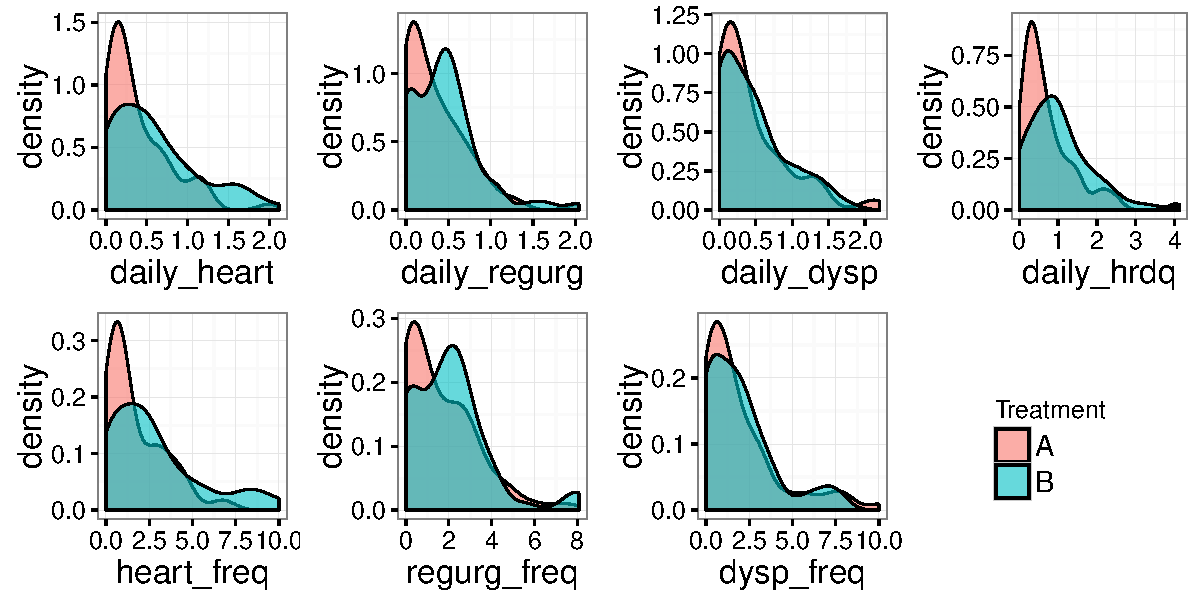
\includegraphics[width = \textwidth]{fig/clinical_distr.pdf}
\caption{Distribution of each endpoint for the two treatments A and B}
\label{fig:clinical_distr}
\end{figure}

%
%\begin{center}
%\begin{table}[ht]
\centering
\begin{tabular}{r|p{1.2in}p{1.2in}p{1.2in}p{1.2in}}
  \hline
 & Parametric ANCOVA & Stratified permutation & LM permutation & Residual permutation \\ 
  \hline
heart\_freq & 0.035 & 0.006 & 0.080 & 0.082 \\ 
  regurg\_freq & 0.136 & 0.118 & 0.280 & 0.220 \\ 
  dysp\_freq & 0.565 & 0.948 & 0.616 & 0.592 \\ 
  daily\_heart & 0.032 & 0.004 & 0.056 & 0.068 \\ 
  daily\_regurg & 0.142 & 0.174 & 0.286 & 0.246 \\ 
  daily\_hrdq & 0.043 & 0.012 & 0.088 & 0.098 \\ 
  daily\_dysp & 0.582 & 0.810 & 0.756 & 0.722 \\ 
   \hline
\end{tabular}
\caption{Comparison of p-values from four tests, for each continuous endpoint.} 
\label{tab:clinical_pvalues}
\end{table}

%\end{center}

\begin{table}[]
\centering
\label{tab:clinical_pvalues}
\begin{tabular}{l|cccc}
Endpoint      & \multicolumn{1}{l}{ANCOVA} & \multicolumn{1}{l}{\begin{tabular}[c]{@{}l@{}}Stratified\\ Permutation\end{tabular}} & \multicolumn{1}{l}{\begin{tabular}[c]{@{}l@{}}LM\\ Permutation\end{tabular}} & \multicolumn{1}{l}{\begin{tabular}[c]{@{}l@{}}Freedman-\\ Lane\end{tabular}} \\ \hline
heart\_freq   & 0.035                      & 0.006                                                                                & 0.080                                                                        & 0.082                                                                        \\
regurg\_freq  & 0.136                      & 0.118                                                                                & 0.280                                                                        & 0.220                                                                        \\
dysp\_freq    & 0.565                      & 0.948                                                                                & 0.616                                                                        & 0.592                                                                        \\
daily\_heart & 0.032                      & 0.004                                                                                & 0.056                                                                        & 0.068                                                                        \\
daily\_regur  & 0.142                      & 0.174                                                                                & 0.286                                                                        & 0.246                                                                        \\
daily\_hrdq   & 0.043                      & 0.012                                                                                & 0.088                                                                        & 0.098                                                                        \\
daily\_dysp   & 0.582                      & 0.810                                                                                & 0.756                                                                        & 0.722                                                                        \\
\hline
\end{tabular}
\caption{Comparison of p-values from four tests, for each continuous endpoint.} 
\end{table}

\section{Discussion}\label{sec:discussion}



This paper adds to the literature comparing parametric and nonparametric tests.
On the one hand, some argue that violations of parametric test assumptions necessitate the use of permutation methods.
\cite{ludbrook_why_1998} point out that medical trials rarely follow the population sampling model implicit in parametric methods.
Many people recommend using permutation tests in place of the usual parametric tests for typical analyses, such as ANOVA and generalized linear models (\cite{still_approximate_1981, winkler_permutation_2014}).
They argue that there are a myriad of ways that the data may violate the necessary assumptions for the test, and so permutation tests are more robust.

However, parametric and nonparametric tests seem to perform similarly when compared side-by-side in simulations, even when data violate the assumptions of the parametric method.
Medical trials often use Likert scales to score pain or symptom severity, resulting in discrete data that does not match the normality assumptions of parametric tests.
However, \cite{winter_five-point_2010} found that the two sample $t$ test and Mann-Whitney test had comparable Type I and II error rates for five-point Likert scale data, suggesting that the violation of normality does not entirely invalidate the parametric test.
\cite{vickers_parametric_2005} compared the parametric ANCOVA to the Mann-Whitney rank test in the context of randomized experiments, finding that except in extreme situations, ANCOVA was more powerful than the nonparametric test.
Most similar to our question of study, \cite{anderson_empirical_1999} found little difference between several permutation tests for coefficients in a linear model alongside the parametric $t$ test.
In these situations, the permutation test strengthens conclusions by giving evidence that the parametric test is robust to departures from its assumptions.

Our results match those of \citet{vickers_parametric_2005} and \citet{anderson_empirical_1999}, where parametric ANCOVA and regression-based $t$ tests performed the same or better than the comparable nonparametric tests.
We simulated a variety of data-generating processes, ranging from the ideal case when all assumptions are met, 
to the case when data are non-normal, discrete, or skewed.
In the supplementary simulation files, we also considered data with other possible issues such as heterogeneous treatment effects and unequal sample sizes.
The linear regression-based tests, both the parametric ANCOVA and the permutation tests, suffered a loss of power when the ANCOVA assumptions were violated.
However, the tests remained comparable to each other.
It is a matter of taste which test one chooses for their experiment: while the parametric test may be robust to violations of its assumptions, it is somewhat reassuring that the permutation test can exactly match the randomization that was done while making no distributional assumptions.
Applying a linear model based permutation test as a secondary analysis can give insight into how ANCOVA results depend on the method's assumptions
(making it conservative, anti-conservative, or not systematically affecting the $p$-value in a particular direction),
and give evidence that inferences based on ANCOVA are reliable.

Permutation tests do not come entirely free of assumptions, though: 
subjects must be exchangeable if we generate the permutation distribution assuming that all possible allocations of treatment which preserve the number of treated units are equally likely.
\cite{romano_behavior_1990} warns against using permutation tests naively if items are not truly exchangeable. 
For instance, he points to the case where observations have unequal variances.  
This is a problem in practice as one cannot observe errors; it is a leap of faith to assert that they are homogeneous and therefore exchangeable.
\cite{boik_fisherpitman_1987} illustrates this phenomenon using the traditional $F$ test and its permutation counterpart, 
and demonstrates by simulation that the latter has larger than nominal level when the error variances are unequal.
Randomized experiments mitigate this problem: by definition, treatment assignment is statistically independent of all other variables (possibly conditioning on strata).

It is important to note that the permutation tests described here are exact only in the context of randomized experiments.
Treatment is assigned at random and is therefore statistically independent of the covariates $X$ and the errors $\varepsilon$.
In observational studies, treatment may be associated with $X$, $\varepsilon$, or both, often in a way that is difficult or impossible to model.
The statistical independence guaranteed by randomized experiments enables us to construct permutation distributions while holding $X$ fixed.
When exchangeability doesn't hold, we cannot disentangle the effect of $Z$ from the effect of $X$.
One must provide evidence that variables in observational studies are exchangeable in order to achieve an approximately exact test.
The onus is on the researcher to make the case that the variable being permuted is uncorrelated with the other variables being held fixed.
This can be done visually using scatterplots and residual plots (see e.g. \cite{freedman_nonstochastic_1983}) and from knowledge of how the data arose and were collected.

One must be mindful of which covariates to include as controls.
Ideally, all covariates related to the outcome are known and observed.
In that case, the coefficient for treatment in a fully saturated linear model (including all covariates and their interactions) is an asymptotically consistent estimate of the average treatment effect (\cite{lin_agnostic_2013}).
It is rare that one knows \textit{all} relevant covariates in practice; failure to control for all relevant variables can introduce bias in some permutation tests.
 \cite{gail_tests_1988} propose a randomization test based on residuals from an exponential family model and find that omitting relevant covariates leads to tests with higher than nominal level.
 
The method of controlling for baseline covariates matters, too.
The naive way is to consider change scores, subtracting baseline measures from the outcome and doing hypothesis testing using the change as the dependent variable.
Our simulations confirm the suggestion of \cite{frison_repeated_1992} to use change scores only when there is a strong correlation between baseline and outcome.
Weak correlations between baseline and outcome occur often in practice, as was the case with our GERD dataset.
When the correlation is weak, the test of change scores may be less powerful than ignoring the baseline altogether.
Instead, we suggest incorporating the baseline in a regression model.
This is more general than using differences;
treating the change scores as the dependent variable is a special case of the linear regression that constrains the coefficient of the baseline measure to be $1$.
The regression approach is more flexible and demonstrably more powerful.



\bigskip
\begin{center}
{\large\bf SUPPLEMENTARY MATERIAL}
\end{center}
All files are also available at \url{https://github.com/kellieotto/ancova-permutations}.

\begin{description}

\item[Gaussian data simulations:] Simulations using Gaussian data in Section~\ref{sec:simulations}, including code and results. (PDF)
\item[Imbalanced design simulations:] Simulations using data with different stratum sizes in Section~\ref{sec:simulations}, including code and results. (PDF)
\item[Skewed data simulations:] Simulations using discrete, skewed data in Section~\ref{sec:simulations}, including code and results. (PDF)
\item[Clinical trial data:] Dataset used in Section~\ref{sec:results} to compare methods. (csv)
\item[README:] Data descriptor file. (txt)
\item[Results:] Detailed explanation, code, and results of comparing methods using the clinical trial dataset in Section~\ref{sec:results}. (PDF)

\end{description}

\bibliographystyle{chicago}

\bibliography{references}
\end{document}
